\documentclass{amsart}
\usepackage{amsmath,amssymb,latexsym}
\usepackage[margin=1in]{geometry}
\usepackage{tikz}

\newtheorem{theorem}{Theorem}
\newtheorem{definition}[theorem]{Definition}
\newtheorem{corollary}[theorem]{Corollary}
\newtheorem{example}[theorem]{Example}
\newtheorem{lemma}[theorem]{Lemma}
\newtheorem{proposition}[theorem]{Proposition}

\newcommand{\bepsilon}{\boldsymbol{\epsilon}}
\newcommand{\fsl}{\mathfrak{sl}}
\newcommand{\ZZ}{\mathbb{Z}}

\makeatletter
\renewcommand{\@evenhead}{\tiny\hfill $\fsl_2$-Tilings Do Not Exist in Higher Dimensions (mostly)\hfill \thepage}

\author{Gr\'egoire Dupont}
\address{}
\email{}

\author{Pierre-Guy Plamondon}
\address{Laboratoire de Math\'ematiques d'Orsay, Univ. Paris-Sud, CNRS, Univ.
Paris-Saclay, 91405 Orsay, France.}
\email{pierre-guy.plamondon@math.u-psud.fr}

\author{Dylan Rupel}
\address{}
\email{}

\author{Salvatore Stella}
\address{}
\email{}

\author{Pavel Tumarkin}
\address{}
\email{}


\title{$\fsl_2$-Tilings Do Not Exist in Higher Dimensions (mostly)}

\begin{document}
  \begin{abstract}
    We show that there exists a unique anti-$\fsl_2$-tiling and no $\fsl_2$-tilings in dimension 3.  We then prove that such tilings do not exist in higher dimensions.
  \end{abstract}
  \maketitle

  \section{$\fsl_2$-Tilings of the Plane}
  The aim of this note is to study higher-dimensional analogues of the following object.
    \begin{definition}[\cite{AssemReutenauerSmith}]
      A bi-infinite array $(a_{ij})_{i,j\in\ZZ}$ with $a_{ij}\in\ZZ_{>0}$ is called an \emph{$\fsl_2$-tiling of $\ZZ^2$} if the entries satisfy the relation
      \begin{equation}\label{eq:sl2 recursion}
        a_{i,j+1}a_{i+1,j}-a_{i+1,j+1}a_{ij}=1.
      \end{equation}
      A bi-infinite array $(b_{ij})_{i,j\in\ZZ}$ with $b_{ij}\in\ZZ_{>0}$  is called an \emph{anti-$\fsl_2$-tiling of $\ZZ^2$} if the entries satisfy the relation
      \begin{equation}\label{eq:anti-sl2 recursion}
        b_{i,j+1}b_{i+1,j}-b_{i+1,j+1}b_{ij}=-1.
      \end{equation}
    \end{definition}
    The notion of an anti-$\fsl_2$-tiling is not actually giving anything new as shown by the following lemma, however this notion will be useful for our considerations in higher dimensions.
    \begin{lemma}
      If $(a_{ij})_{i,j\in\ZZ}$ is an $\fsl_2$-tiling, then taking $b_{ij}=a_{i,-j}$ gives an anti-$\fsl_2$-tiling.
    \end{lemma}
    One should think of the difference between $\fsl_2$-tilings and anti-$\fsl_2$-tilings as viewing the lattice $\ZZ^2$ ``from above'' or ``from below.''
    
    The following result from \cite{AssemReutenauerSmith} was our starting point.
    \begin{theorem}[\cite{AssemReutenauerSmith}]
      There exist infinitely many $\fsl_2$-tilings of $\ZZ^2$.
    \end{theorem}
    
    In fact, it is shown in \cite{AssemReutenauerSmith} that any ``frontier'', or broken line of $1$'s in the plane, can be completed into a unique $\fsl_2$-frieze.  An interpretation of all possible $\fsl_2$-tilings involving triangulations of a polygon with infinitely many vertices was later given in \cite{HolmJorgensen}.

    \begin{example}\label{ex:Fibonacci}
      Consider the $\fsl_2$-tiling $(a_{ij})_{i,j\in\ZZ}$ of $\ZZ^2$ with $a_{ij}=1$ if $i-j\in\{0,1\}$.  Then using \eqref{eq:sl2 recursion} and the well-known recursion $F_{2r-1}F_{2r+3}=F_{2r+1}^2+1$ $(r\ge1)$ for the odd Fibonacci numbers, we see that
      \[a_{ij}=\begin{cases}F_{2r-1} & \text{if $i-j=r\ge1$;}\\F_{-2r+1} & \text{if $i-j=r\le0$;}\end{cases}\]
      where we number the Fibonacci numbers as:
      \[\begin{tabular}{|c|c|c|c|c|c|c|c} $F_1$ & $F_2$ & $F_3$ & $F_4$ & $F_5$ & $F_6$ & $F_7$ & $\cdots$\\\hline 1 & 1 & 2 & 3 & 5 & 8 & 13 & $\cdots$\end{tabular}\]
      The following figure is a section of this tiling. Note the bolded frontier of $1$'s.
      \begin{center}
      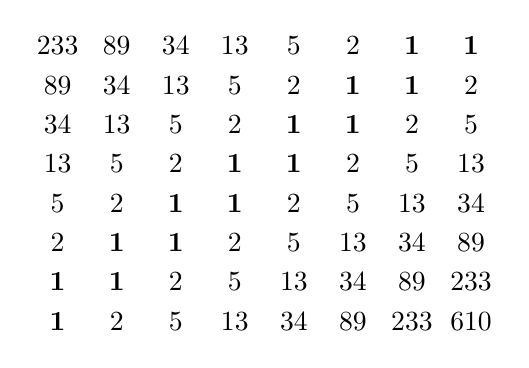
\begin{tikzpicture}
       \draw (0,1) node{$233$} (.75,1) node{$89$} (1.5,1) node{$34$} (2.25,1) node{$13$} (3,1) node{$5$} (3.75,1) node{$2$} (4.5,1) node{${\bf 1}$} (5.25,1) node{${\bf 1}$};
       \draw (0,.5) node{$89$} (.75,.5) node{$34$} (1.5,0.5) node{$13$} (2.25,0.5) node{$5$} (3,0.5) node{$2$} (3.75,0.5) node{${\bf 1}$} (4.5,0.5) node{${\bf 1}$} (5.25,0.5) node{$2$};
       \draw (0,0) node{$34$} (.75,0) node{$13$} (1.5,0) node{$5$} (2.25,0) node{$2$} (3,0) node{${\bf 1}$} (3.75,0) node{${\bf 1}$} (4.5,0) node{$2$} (5.25,0) node{$5$};
       \draw (0,-.5) node{$13$} (.75,-.5) node{$5$} (1.5,-.5) node{$2$} (2.25,-.5) node{${\bf 1}$} (3,-.5) node{${\bf 1}$} (3.75,-.5) node{$2$} (4.5,-.5) node{$5$} (5.25,-.5) node{$13$};
       \draw (0,-1) node{$5$} (.75,-1) node{$2$} (1.5,-1) node{${\bf 1}$} (2.25,-1) node{${\bf 1}$} (3,-1) node{$2$} (3.75,-1) node{$5$} (4.5,-1) node{$13$} (5.25,-1) node{$34$};
       \draw (0,-1.5) node{$2$} (.75,-1.5) node{${\bf 1}$} (1.5,-1.5) node{${\bf 1}$} (2.25,-1.5) node{$2$} (3,-1.5) node{$5$} (3.75,-1.5) node{$13$} (4.5,-1.5) node{$34$} (5.25,-1.5) node{$89$};
       \draw (0,-2) node{${\bf 1}$} (.75,-2) node{${\bf 1}$} (1.5,-2) node{$2$} (2.25,-2) node{$5$} (3,-2) node{$13$} (3.75,-2) node{$34$} (4.5,-2) node{$89$} (5.25,-2) node{$233$};
       \draw (0,-2.5) node{${\bf 1}$} (.75,-2.5) node{$2$} (1.5,-2.5) node{$5$} (2.25,-2.5) node{$13$} (3,-2.5) node{$34$} (3.75,-2.5) node{$89$} (4.5,-2.5) node{$233$} (5.25,-2.5) node{$610$};
       
      \end{tikzpicture}
      \end{center}
    \end{example}

  \section{$\fsl_2$-Tilings in Higher Dimensions}
    \begin{definition}
      Fix $\bepsilon=(\epsilon_{k\ell})_{1\le k<\ell\le n}\in\{\pm1\}^{{n\choose 2}}$.  An array $(a_{i_1,\ldots,i_n})_{i_k\in\ZZ}$ with $a_{i_1,\ldots,i_n}\in\ZZ_{>0}$ is called an \emph{$\bepsilon-\fsl_2$-tiling of $\ZZ^n$} if for each $1\le k<\ell\le n$ we have
      \begin{equation}\label{eq:higher sl2 recursion}
        a_{i_1,\ldots,i_k,\ldots,i_\ell+1,\ldots,i_n}a_{i_1,\ldots,i_k+1,\ldots,i_\ell,\ldots,i_n}-a_{i_1,\ldots,i_k,\ldots,i_\ell,\ldots,i_n}a_{i_1,\ldots,i_k+1,\ldots,i_\ell+1,\ldots,i_n}=\epsilon_{k\ell}.
      \end{equation}
    \end{definition}
    The situation is now different than the $n=2$ case, all the $\bepsilon$-$\fsl_2$-tilings are not necessarily equivalent, however there do remain relations among them.
    \begin{lemma}\label{le:relabel}
      Let $\bepsilon=(\epsilon_{k\ell})_{1\le k<\ell\le n}\in\{\pm1\}^{{n\choose 2}}$ and write $\bepsilon^{(r)}=(\epsilon'_{k\ell})_{1\le k<\ell\le n}\in\{\pm1\}^{{n\choose 2}}$ where $\epsilon'_{k\ell}=-\epsilon_{k\ell}$ if $k=r$ or $\ell=r$ and $\epsilon'_{k\ell}=\epsilon_{k\ell}$ otherwise.  If $(a_{i_1,\ldots,i_n})_{i_k\in\ZZ}$ is an $\bepsilon-\fsl_2$-tiling, then taking $b_{i_1,\ldots,i_n}=a_{i_1,\ldots,-i_r,\ldots,i_n}$ gives an $\bepsilon^{(r)}-\fsl_2$-tiling.
    \end{lemma}
    \begin{lemma}\label{le:constant slices}
      Let $\epsilon=\pm1$ and assume $(a_{i_1,i_2,i_3})_{i_k\in\ZZ}$ is an $(\epsilon,\epsilon,\epsilon)-\fsl_2$-tiling of $\ZZ^3$.  Then for any $r\in\ZZ$ the set $\{a_{i_1,i_2,i_3}:i_1+i_2+i_3=r\}$ consists of a single element.
    \end{lemma}
    \begin{proof}
      To see this we compute $a_{i_1+1,i_2+1,i_3+1}$ in terms of $a_{i_1,i_2,i_3}, a_{i_1+1,i_2,i_3}, a_{i_1,i_2+1,i_3}, a_{i_1,i_2,i_3+1}$ in three different ways.  For simplicity of notation we set:
      \[a_{i_1,i_2,i_3}=a,\quad\quad a_{i_1+1,i_2,i_3}=x,\quad\quad a_{i_1,i_2+1,i_3}=y,\quad\quad a_{i_1,i_2,i_3+1}=z.\]
      The following picture will be useful.
      \begin{center} 
      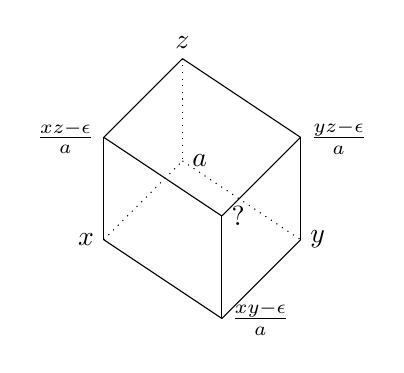
\begin{tikzpicture}
       \draw (0,0) -- ++(1,1)  node[above] {$z$} ;
       \draw (0,0) node[left] {$\frac{xz-\epsilon}{a}$} ;
       \draw (0,0) -- ++(0,-1.3) node[left] {$x$} ;
       \draw [dotted] (1,1) -- ++(0,-1.3) node[right] {$a$};
       \draw [dotted] (0,-1.3) -- ++(1,1) ;
       \draw (0,0) -- ++(1.5,-1) node[right] {?} ;
       \draw (1,1) -- ++(1.5,-1) node[right] {$\frac{yz-\epsilon}{a}$};
       \draw (0,-1.3) -- ++(1.5,-1) node[right]{$\frac{xy-\epsilon}{a}$};
       \draw [dotted] (1,-.3) -- ++(1.5,-1) ;
       \draw (1.5,-1) -- ++(0,-1.3) ;
       \draw (1.5,-1) -- ++(1,1) ;
       \draw (1.5,-2.3) -- ++(1,1) ;
       \draw (2.5,0) -- ++(0,-1.3) node[right]{$y$} ;
      \end{tikzpicture}      
      \end{center}
      Using \eqref{eq:higher sl2 recursion} three times we get
      \[a_{i_1+1,i_2+1,i_3}=\frac{xy-\epsilon}{a},\quad\quad a_{i_1,i_2+1,i_3+1}=\frac{yz-\epsilon}{a},\quad\quad a_{i_1+1,i_2,i_3+1}=\frac{xz-\epsilon}{a}.\]
      Then applying \eqref{eq:higher sl2 recursion} three more times gives
      \begin{align*}
        a_{i_1+1,i_2+1,i_3+1} 
        &= \frac{a_{i_1+1,i_2+1,i_3}a_{i_1+1,i_2,i_3+1}-\epsilon}{a_{i_1+1,i_2,i_3}}=\frac{xyz}{a^2}-\epsilon\frac{y+z}{a^2}-\epsilon\frac{a^2-\epsilon}{a^2x};\\
        &= \frac{a_{i_1+1,i_2+1,i_3}a_{i_1,i_2+1,i_3+1}-\epsilon}{a_{i_1,i_2+1,i_3}}=\frac{xyz}{a^2}-\epsilon\frac{x+z}{a^2}-\epsilon\frac{a^2-\epsilon}{a^2y};\\
        &= \frac{a_{i_1+1,i_2,i_3+1}a_{i_1,i_2+1,i_3+1}-\epsilon}{a_{i_1,i_2,i_3+1}}=\frac{xyz}{a^2}-\epsilon\frac{x+y}{a^2}-\epsilon\frac{a^2-\epsilon}{a^2z}.
      \end{align*}
      It follows that $\frac{x-y}{a^2}=\frac{a^2-\epsilon}{a^2x}-\frac{a^2-\epsilon}{a^2y}$ or $(xy+a^2-\epsilon)(x-y)=0$.  But $xy+a^2-\epsilon\ge1$ since $a,x,y\ge1$, hence $x=y$.  Similarly $y=z$ and the result follows.
    \end{proof}
    
    We now come to our first main result: in dimension $3$, an ``infinite staircase'' of $1$'s yields the only possible $(-1,-1,-1)-\fsl_2$-tiling.

    \begin{theorem}
      For $\bepsilon=(-1,-1,-1)$, there exists a unique (up to translation) $\bepsilon-\fsl_2$-tiling of $\ZZ^3$.
    \end{theorem}
    \begin{proof}
      Assume $(a_{i_1,i_2,i_3})_{i_k\in\ZZ}$ is a $(-1,-1,-1)-\fsl_2$-tiling of $\ZZ^3$.  Pick $i_1,i_2,i_3$ with $a_{i_1,i_2,i_3}$ minimal.  Applying \eqref{eq:higher sl2 recursion} gives
      \[a_{i_1+1,i_2,i_3}a_{i_1,i_2-1,i_3}=a_{i_1,i_2,i_3}a_{i_1+1,i_2-1,i_3}+1=a_{i_1,i_2,i_3}^2+1,\]
      where we applied Lemma~\ref{le:constant slices} in the last equality.  If $a_{i_1,i_2,i_3}>1$, this implies $a_{i_1+1,i_2,i_3}<a_{i_1,i_2,i_3}$ or $a_{i_1,i_2-1,i_3}<a_{i_1,i_2,i_3}$, contradicting minimality, so we must have $a_{i_1,i_2,i_3}=1$.  This implies $\{a_{i_1+1,i_2,i_3},a_{i_1,i_2-1,i_3}\}=\{1,2\}$.  Without loss of generality we will assume $a_{i_1+1,i_2,i_3}=2$ and $i_1+i_2+i_3=1$.  Then applying \eqref{eq:higher sl2 recursion} repeatedly shows that $a_{j_1,j_2,j_3}$ with $j_1+j_2+j_3=r\ge1$ is exactly the $r^{th}$ odd Fibonacci number $F_{2r-1}$, see Example~\ref{ex:Fibonacci}.  Similarly one sees that $a_{j_1,j_2,j_3}$ with $j_1+j_2+j_3=r\le0$ is the odd Fibonacci number $F_{-2r+1}$.
    \end{proof}

Our second main result is about the absence of other types of tilings.

    \begin{theorem}\label{th:nonexistence}
      For $\bepsilon=(1,1,1)$, there does not exist an $\bepsilon-\fsl_2$-tiling of $\ZZ^3$.
    \end{theorem}
    \begin{proof}
      Assume $(a_{i_1,i_2,i_3})_{i_k\in\ZZ}$ is a $(1,1,1)-\fsl_2$-tiling of $\ZZ^3$.  Pick $i_1,i_2,i_3$ with $a_{i_1,i_2,i_3}$ minimal.  Applying \eqref{eq:higher sl2 recursion} gives
      \[a_{i_1+1,i_2,i_3}a_{i_1,i_2-1,i_3}=a_{i_1,i_2,i_3}a_{i_1+1,i_2-1,i_3}-1=a_{i_1,i_2,i_3}^2-1,\]
      where we applied Lemma~\ref{le:constant slices} in the last equality.  But this implies $a_{i_1+1,i_2,i_3}<a_{i_1,i_2,i_3}$ or $a_{i_1,i_2-1,i_3}<a_{i_1,i_2,i_3}$, contradicting minimality.
    \end{proof}

    \begin{corollary}
      For $n\ge4$, there is no $\bepsilon\in\{\pm1\}^n$ for which there exists an $\bepsilon-\fsl_2$-tiling of $\ZZ^n$.
    \end{corollary}    
   \section*{Acknowledgements}
   These results were obtained while we were taking part in the Conference on
Cluster Algebras and Representation Theory at the KIAS in Seoul, South Korea. We would like to thank the organizers of that meeting for the stimulating environment they provided.
    
\begin{thebibliography}{99}
 \bibitem{AssemReutenauerSmith}  	Ibrahim Assem, Christophe Reutenauer and David Smith, \emph{Friezes}, Advances in Mathematics {\bf 225} (2010) 3134-3165.
 \bibitem{HolmJorgensen} Thorsten Holm and Peter J\o rgensen, \emph{To appear?}.
\end{thebibliography}
  
\end{document}
